% This version of CVPR template is provided by Ming-Ming Cheng.
% Please leave an issue if you found a bug:
% https://github.com/MCG-NKU/CVPR_Template.

\documentclass[final]{cvpr}
\usepackage[utf8]{inputenc}
\usepackage{times}
\usepackage{epsfig}
\usepackage{graphicx}
\usepackage{amsmath}
\usepackage{amssymb}
\usepackage{fancyhdr}
\usepackage{relsize}

% Include other packages here, before hyperref.

% If you comment hyperref and then uncomment it, you should delete
% egpaper.aux before re-running latex.  (Or just hit 'q' on the first latex
% run, let it finish, and you should be clear).
\usepackage[pagebackref=true,breaklinks=true,colorlinks,bookmarks=false]{hyperref}


\def\cvprPaperID{****} % *** Enter the CVPR Paper ID here
\def\confYear{CVPR 2021}
%\setcounter{page}{4321} % For final version only


\begin{document}

%%%%%%%%% TITLE
\title{Crypto return prediction}

\author{Siddartha Marella\\
UNI: sm4940\\
{\tt\small sm4940@columbia.edu}
% For a paper whose authors are all at the same institution,
% omit the following lines up until the closing ``}''.
% Additional authors and addresses can be added with ``\and'',
% just like the second author.
% To save space, use either the email address or home page, not both
\and
Varun Jasti\\
UNI: vj2552\\
{\tt\small vj2552@columbia.edu}
}

\maketitle


%%%%%%%%% BODY TEXT
\section{Abstract}
The Crypto currencies are volatile assets that are challenging to accurately predict but as potentially a dominant form of currency in the future, it is highly valuable to be able to predict them accurately. In this paper, Effective features are explored that can encompass the socio-political factors through using multiple popular cryptocurrencies analysis along with Tweet Volume Analysis and Twitter sentiment analysis. Experiments were run to identify the correlation between 14 different popular currencies and how to effectively use them for cryptocurrency prediction. Sensitivity analysis of tweets was done to check its effectiveness as a feature in predicting returns of cryptocurrency. Experiments were run to identify the best set of features and models to predict the crypto returns. Results show that not only deep learning models like LSTM but linear regressors like SGD can be effective when essential features are provided and the constraints are fixed like prediction after a certain amount of time(like 15 mins). Results show that the effective features are volatile for crypto prediction and the model trained in the one-time frame(Q1 2021) will not be as effective in another (Q2 2021). Hence, Dynamic feature engineering and model selection become important. In this paper, dynamic model selection is done through effective use of AutoML techniques and it promises better accuracy and can cater to a wide range of constraints. The pipeline has been established to fetch the real-time crypto values of the 14 different popular cryptocurrencies and tweets which are used for prediction. Even to further reduce the risk of investors investing in cryptocurrencies, Portfolio analysis was performed on 14 different cryptocurrencies to create an algorithm that generates a portfolio of different currencies taking the user constraints on risk and returns. A web app is created where the user can track the cryptocurrencies and generate his choice of portfolio based on his needs. Even to further reduce the risk of investors investing in cryptocurrencies, Portfolio analysis was done on 14 different cryptocurrencies to create an algorithm that generates a portfolio of different currencies taking the user constraints on risk and returns. A web app is created where the user can track the cryptocurrencies and generate his choice of portfolio based on his needs.

\section{Introduction}

Cryptocurrencies are traded at a volume of 40 billion dollars every day. It is potentially the future currency that overtakes the dollar. It is one of the most volatile assets and can give investors huge profits and crushing losses as well. As it is dependent on socio-political factors around the world, it becomes a challenging and valuable problem to predict the returns.

The objective of this paper is to discuss effective ways of feature engineering for crypto prediction and tries methods like using 14 different popular crypto currencies to read the trend for predicting a single crypto currency, Twitter sentiment analysis was also done to check its impact on the price of the crypto value. Then, the paper discusses about model selection for crypto price prediction where different ML models from literature like LSTM, SGD and linear regressor are individually trained. Then, it discusses the results of dynamic model selection where H2O AutoML tool is used to train and identify the best model for different constraints like period of prediction (15mins to 1 day)and available relevant training data set(1 month to 1 year). Then, the paper discusses the model of a crypto asset portfolio algorithm for the 14 different crypto currencies which reduces the risk of investing on volatile crypto currencies and can generate a portfolio for the investor's desired return against risk. Then, paper discusses the pipeline creation which feeds in real-time crypto and tweets information. Finally, the paper discusses the web app where an investor can track multiple crypto prices and generate his desired portfolio.

 The project is inspired by a live Kaggle competition \cite{kaggle}. This competition is sponsored by G-Research. It is a European finance research firm that has provided crypto data from 2018 of 14 different cryptocurrencies which include the major ones like BTC, ETH, Doge, etc. Initially, time series analysis was done to identify the relation between these different currencies and it is found that these currencies show a strong relation in terms of the trend but have poor correlation in terms of seasonality. Then the cross correlation analysis was done between these currencies to identify if other cryptocurrencies can be used as features for the prediction of a single cryptocurrency. The results show that the correlation is highly variable and can range from very strong correlation to no correlation at all. The twitter analysis also yielded similar results as the correlation was mixed. To obtain a baseline model, experiments were done on different ML algorithms from the scikit library and also ran the LSTM model using TensorFlow. The results show that these models are temporally effective and have high variance and will not be as effective in a different period. For the Twitter sentiment analysis, we have used spark streaming and tweepy library to access Twitter API and read the number of counts of crypto keywords from the set of crypto words we have created. The result of the sentiment analysis found that there is a correlation with prices going up and down between how the tweets are distributed based on the sentiment. However, the correlation becomes weaker with regards to distribution of negative tweets whenever there is a sudden crash in the market. As a result, the findings are mixed as this is found to be useful as an additional piece of supplementary information in the overall picture of the model instead of being main part of model due there being a drawback along with the positives. Google cloud storage bucket is used for storage. All the above results showed a need of dynamic model that can counter the over-fitting and deliver good accuracy. H2O autoML tool is used to train different crypto currencies data temporally and the results show a increased and consistent accuracy across the time period and for different crypto currencies. The tool also highlighted the need of a dynamic model as the best model was from different algorithms(deeplearning, GBM, stacked ensemble) in different periods. Then portfolio analysis was done using Markowitz hypothesis on the 14 different crypto currencies to reduce the risk of the investor in achieving the desired returns. It uses quadratic optimization to identify the low risk portfolios for a desired return. Finally, a web app is created using plotly dash, that can be used to track these 14 different currencies and to identify the weights of an efficient portfolio for a maximising the returns at a desired risk for an investor.



%-----------------------------------------------------------
\section{Related work}
The "Cryptocurrency Price Prediction Using Tweet Volumes and Sentiment Analysis" paper, explains how analysis methods of Twitter Sentiment Analysis, Google Trends analysis, and Tweet volume analysis were tried.~\cite{Alpher} The Twitter Sentiment Analysis method was not very accurate in being able to predict the future values of the cryptocurrency as the sentiment did not act as a good indicator of future price prediction as positive sentiment was there when the price went both up and down. The Google Trends analysis method was showing fairly steady accuracy in predicting future prices of cryptocurrency based on the data provided by Google Trends. This was showing a good correlation with the Pearson R-value of 0.817. The Tweet volume analysis method was showing best of all the three methods in terms of being able to predict the future prices of the cryptocurrency. The volume of tweets for the cryptocurrency was showing the best correlation with cryptocurrency prices as it had a Pearson R-value of 0.841. Based on this, we have decided to tailor our approach to focusing on using both the Tweet Volume Analysis method and the Twitter Sentiment Analysis method for our project by counting the number of hashtags related to the cryptocurrency we are monitoring to get a volume count along with sentiment analysis to monitor and supplement our prediction of future cryptocurrency prices. We were initially planning on doing a Twitter Sentiment Analysis to see if we can do future cryptocurrency price predictions but decided it would be better to adjust our focus to include a combination of the Tweet Volume Analysis method along with the Twitter Sentiment Analysis based on the results of this paper. This is due to the Tweet Volume Analysis giving us a quantitative measure while also being able to qualitatively determine the price correlation with Twitter Sentiment Analysis as an addition input into the data even though Twitter Sentiment Analysis might not give the best quantitative results. Knowing the public sentiment can be very useful in making key determinations of certain factors which might influence the cryptocurrency prices. Overall, this paper helped us evaluate the benefits and drawbacks of pursuing each method and come to a conclusion on one of the main methods we wanted to proceed with for final analysis.~\cite{Alpher}

\par We did realize that Tweet Volume Analysis and Twitter Sentiment Analysis alone were not enough to create a robust prediction model for our cryptocurrency price prediction as Tweet volume and Twitter sentiment alone are not enough to account for any sudden market changes that might happen. That is why we decided to look at deep learning modeling options as our other main method to supplement our Tweet Volume Analysis. Having a type of deep learning model is important for cryptocurrency price prediction as we would need our model to be able to cope with sudden volatile market changes that might make the price go exponentially up or down. It is not enough to have a model or analysis method that works only under ideal market circumstances as the market is anything but ideal so adaptability is the main trait to be considered. Based on this, we decided to go with the LSTM Model approach to supplement our Tweet Volume Analysis. "An LSTM-Method for Bitcoin Price Prediction: A Case Study Yahoo Finance Stock Market" paper discusses how the LSTM approach provides high accuracy predictions for the Bitcoin cryptocurrency prices.~\cite{inproceedings} LSTM is a deep learning model which has memory management that optimizes the predictions based on the time series and it's a model which can self-improve as more training data is input into the model. The paper shows how the LSTM model ends up with Bitcoin currency predictions that have low Root Mean Square Error when compared to actual values. Root Mean Square Error is a reliable metric as it normalizes the accuracy to give an idea of how robust the model is. Based on this, we decided to go ahead with having LSTM as our model to supplement the Tweet Volume Analysis and Twitter Sentiment Analysis we are doing to create an overall system that is able to predict future cryptocurrency values with higher accuracy.~\cite{inproceedings}

\par Based on the two papers we have reviewed, we decided it was best to make our unique approach taking into account the findings of these papers. Using the Tweet Volume Analysis and Twitter Sentiment Analysis in conjunction with the LSTM model has created some interesting results and to complement these methods we tried out different machine learning model techniques and creating crypto trend functions to see if it gives any strong correlation

Kaggle has been a great source of lot of articles, that provided us good time series analysis methods, insights into performing EDA for our data. We have used methods like calculating stationary nature of different attributes. learnt on time series analysis methods on identifying correlation trend and seasonality analysis.\cite{kaggle}
\section{Data}

Data is from the Kaggle competition which is designed for crypto prediction which has high-frequency data from 2018 to September 2021. It has 14 different currencies for most of the period mentioned, which include, bitcoin cash, Binance, bitcoin, EOS, ETH classic, ETH, Litecoin, Monero, Stellar, Cardano, IOTA, TRON, maker, and Dogecoin. The time-series data is generally available every 10 sec for most of the time. It has the common attributes, High, Low, Volume, Open and Close. Along with these attributes, 'count' is the number of trades in the last interval. VWAP is the attribute that tells us the average price after the weighted volume. Another attribute is Target, which is designed for prediction, where it is calculated as residual log returns for the currency over the 15min horizon. It is calculated using the formula, $$R(t) = log(P(t+16)/P(t+1))$$
\\
As the cryptocurrencies are hugely correlated, the target variable is created with linear residualization, targeted to remove the market impact on each of the assets. The weights of each currency are created with expertise and the market return is given by  $$M(t) = \sum_a \frac{w_a * R_a}{w_a}$$
The rolling average function is used for normalization, if rolling average function is RA, then
$$Target = R_a - \frac{RA(M*R_A)}{RA(M^2)}*M$$

The open, high, close and low and Target data had a few missing values which were removed. This could be done as the data is high frequency where each row corresponds approximately to 10secs. 

As the close prices need to be used for model training,they have to be stationary for a better performance. To verify the stationary nature of the data, "Augmented Dickey-Fuller" test was performed. The results show that all of the currencies are non-stationary and some even with a very high p-value.For the full list refer:\ref{tab:ADF-C}

\begin{table}[h!]
\centering
 \begin{tabular}{ |p{2.5cm}|p{1.5cm}|p{1.5cm}|}
 \hline
 \multicolumn{3}{|c|}{\textbf{ADF - stationary test}} \\
 \hline
 Currency & Stationary & p-value \\
 \hline
 Bitcoin  & FALSE & 0.62 \\
 \hline
 Ethereum  & FALSE & 0.14 \\
 \hline
  \end{tabular}
  \caption{ADF- Stationary test for close prices in Q1-2021.}
 \label{tab:ADF}
\end{table}

All the columns of the data are converted to their log returns to make them stationary and it is observed that all the currencies close prices have become stationary.For the full list refer:\ref{tab:ADF1-C}


\begin{table}[h!]
\centering
 \begin{tabular}{ |p{2.5cm}|p{1.5cm}|p{1.5cm}|}
 \hline
 \multicolumn{3}{|c|}{\textbf{ADF - stationary test}} \\
 \hline
 Currency & Stationary & p-value \\
 \hline
 Bitcoin  & TRUE & 0 \\
 \hline
 Ethereum  & TRUE & 0  \\
 \hline

  \end{tabular}
  \caption{ADF- Stationary test for close prices in Q1-2021 after log-return calculation.}
 \label{tab:ADF1}
\end{table}
\section{Methods}

\subsection{Feature selection}
\subsubsection{Crypto assets}

We know that features are very important for our objective of creating a good model. We have tried a new method of using different crypto currency values to predict each crypto currency like use the open,close,high and low values of Ethereum along with bitcoin to predict the bitcoin future returns. To estimate which crypto values are more closely correlated, we have created a correlation map of all the 14 crypto currencies for 1st\ref{fig:all1} and 2nd\ref{fig:all2} quarters of 2021.  When we compare the correlation between 1st and 2nd quarters of 2021, we can see that the correlation between the bitcoin and the ethereum is very high in the second quarter of 2021 which we know is the period where all the cryto currencies where rising in the market but when we look at the 1st quarter the relation between the two currencies is low.

\begin{figure}[h!]
\begin{center}
\caption{correlation among all crypto currencies in quarter 1 of 2021}
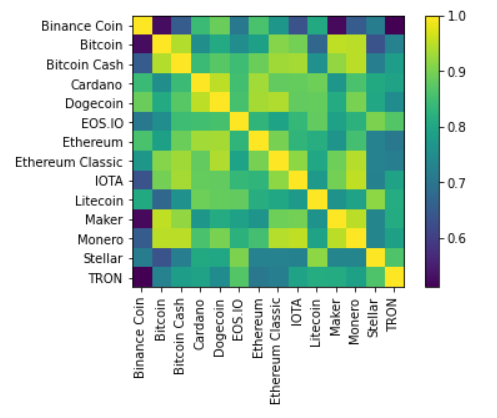
\includegraphics[width=0.8\linewidth]{latex/cor1.png}
\end{center}
\label{fig:all1}
\end{figure}

\begin{figure}[h!]
\begin{center}
\caption{correlation among all crypto currencies in quarter 2 of 2021}
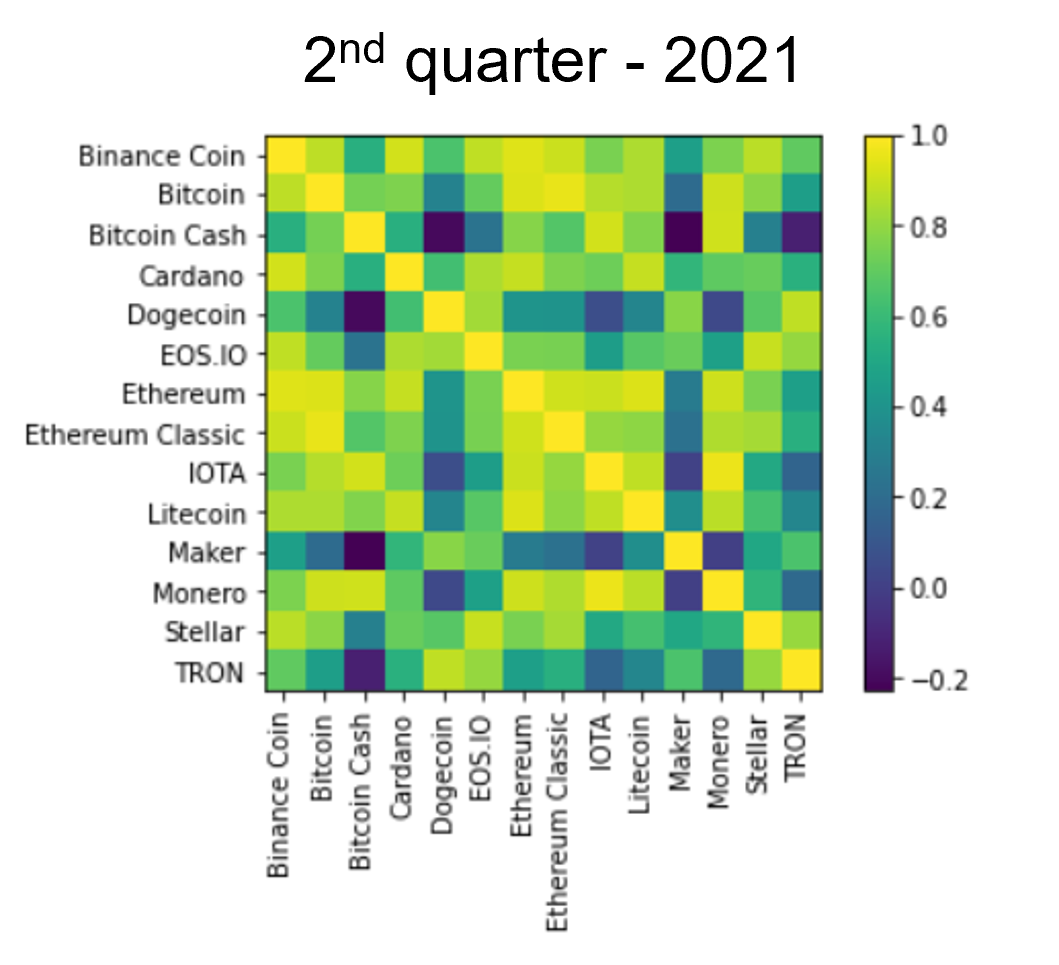
\includegraphics[width=0.8\linewidth]{latex/cor2.png}
\end{center}
\label{fig:all2}
\end{figure}

If we extend our analysis to a single quarter between the Bitcoin and Ethereum, we can see that correlation is highly dynamic\ref{fig:btceth} ranging from 0 to 1. But as can be seen from the heat map\ref{fig:all2} the correlation was clearly evident. 

\begin{figure}[h!]
\begin{center}
\caption{correlation between BTC and ETH in quarter 1 of 2021}
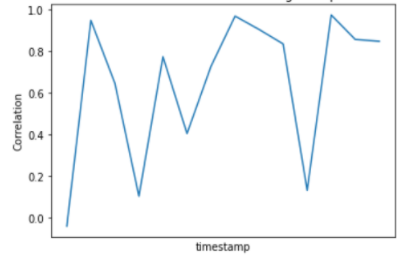
\includegraphics[width=0.8\linewidth]{latex/btc_eth_cor.PNG}
\end{center}
\label{fig:btceth}
\end{figure}

To identify the usefulness of other currencies in predicting bitcoin prices, we have used the SGD regression model to use both the attributes from bitcoin and ethereum for the bitcoin prediction\ref{fig:btcethpred} and we observed no improvement in the accuracy. Although, we are sure that there is intelligence that can be extracted we can't see a way right now and hence this method is discarded for the future runs.

\begin{figure}[h!]
\begin{center}
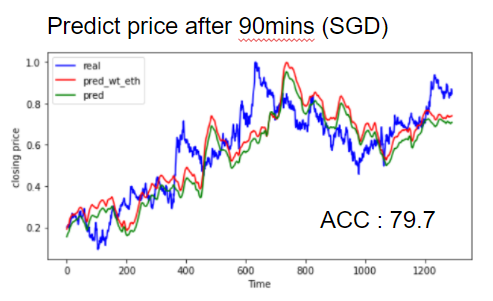
\includegraphics[width=0.8\linewidth]{latex/sgd.png}
\end{center}
   \caption{Bitcoin prediction using both bitcoin and ethereum attributes }
\label{fig:btcethpred}
\end{figure}

When we have used different attributes as features, we have seen that the normal price attributes like low,close, open, high have a higher variance explanation compared to other attributes like VWAP and target. Hence they were only used in the later runs.

\subsubsection{Twitter feed}
We have used the Twitter API through the tweepy package from Python to interact with Twitter. This gives us the ability to stream the twitter data we are looking for in order to check its efficacy as a feature and to perform the Twitter Sentiment Analysis and the Tweet Volume Analysis. Especially regarding the Twitter Sentiment Analysis, we use the NLTK library from Python to quantitatively score the sentiment and assign each tweet a quantitative value to be used for distribution when doing the mathematical analysis regarding correlation. We also use the CryptoCompare API to stream the live cryptocurrency prices to do our correlation analysis regarding the Tweet Volume and the Sentiment. We figured this was the best method to account for external social-political factors into our model that might affect the cryptocurrency prices because Twitter is a commonly used social media platform where a lot of information about cryptocurrencies are passed around. This was expected to help us encompass social factors but when observed that this doesn't have a clear correaltion with the crypto prices, it is discarded to avoid increase of variance in the model.

\subsection{Model selection}
Experiments were run to identify the best model for crypto prediction.
\subsubsection{LSTM}
Literature points towards LSTM as the best predictive model for the crypto returns. So, we have replicated the method for bitcoin prediction and have seen that the model performs very well for predicting short term in the future like after 1 unit of training data frame time(could be a minute or a day). but doesn't perform well when predicting well ahead in the future like 30 units of training data frame time period as can be seen from the results in the Experiments section.
\subsubsection{Linear Regression models}
 We have tried a new approach of using simple linear regression models to predict the crypto return well ahead in the future as LSTM was unable to perform well.\ref{fig:LSTM90} and have found that simple linear model performs better compared to LSTM prediction\ref{fig:linear90}
 
 
 
 \subsection{Dynamic Model}
 
 As can be seen in the experiments\ref{fig:h2obtc}, After training different models on the crypto data set, we have observed that to have the best accuracy we can afford a high vairance model but we need to train a different model every time to have consistently high accuracy. So, we have approached a new method of having a dynamic model that trains for every new time window. We have utilised the H2O AutoML tool that runs data through different algorithms like gradient boositng machine, multi-layer perceptron, distributed random forest, generalised linear models and stacks all the best performing models to create ensemble models. It performs a hyper parameter grid search to identify the best performing model. 
 
 The experiment of predicting bitcoin's next close price was performed by giving last six months data as input for training and testing on the data for the next 30 units of time frame(30 days here) and have obtained a very good accuracy of 95.3\%.\ref{fig:h2obtc}. This is significantly higher than all the individual models that were trained. The best model generated is a multi layer perceptron with 5 layers, all the middle layers have 50 rectifier units with a drop out rate of 40 and has selected linear as the activation function for the output layer. This shows that hyperparameter grid search is important to identify better performing models.
 
\begin{figure}[h!]
\begin{center}
\caption{Bit coin price prediction using H2O}
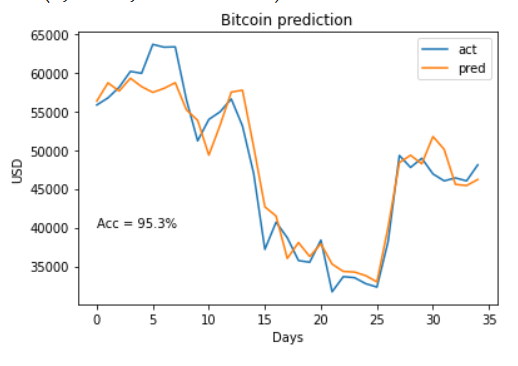
\includegraphics[width=0.8\linewidth]{latex/H2O_btc.PNG}
\end{center}
\label{fig:h2obtc}
\end{figure}
 
\subsection{Portfolio analysis}

As crypto currencies are highly volatile, it can provide investors a means to make huge profits and at the same time holds a huge risk of incurring huge losses. To minimize the risk we have used the markowitz approach to identify the least risk portfolios that can deliver desired return. This is an already established hypothesis in stock market and there is new literature showing how adding crypto to existing portfolio is beneficial.~\cite{portfolio}

We have extended this method to all cryptocurrency portfolio that would distribute the investment among the 14 different cryptocurrency to minimize the risk for the same amount of desired return. The algorithm uses past 1 year data to calculate the risk (Covariance matrix of assets) and uses the daily returns across one year to calculate the average return. Then quadratic optimization is performed to solve for the minimum risk for the required return. If there are n crypto currencies and W is weight vector that distributes the investment and $\Omega$ is the co-variance matrix and $\mu$ is the vector of mean returns  generated from the past crypto data for 1 year then the total risk and return are given by $$\mu_{net} = W*\mu$$ $$\sigma^2 = W^T\Omega W $$

We also know that sum of the weights has to be 1, by solving these we get the required portfolio for a desired return. Portfolio analysis has been done on the 14 crypto assets as shown in here\ref{fig:port}. 

\begin{figure}[h!]
\begin{center}
\caption{Portfolio using all 14 different currencies}
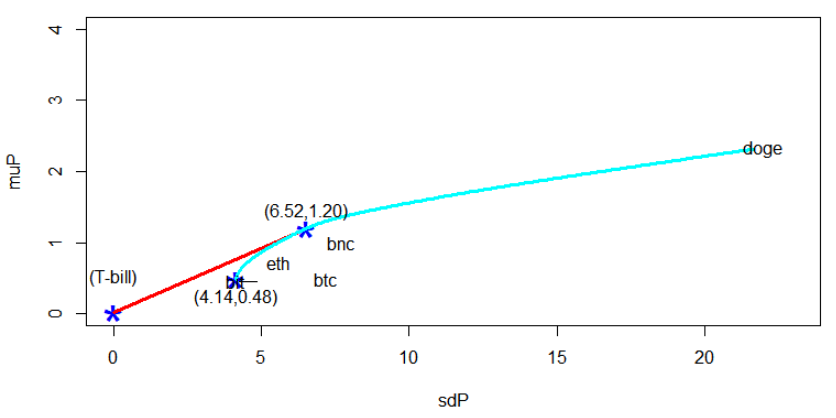
\includegraphics[width=0.8\linewidth]{latex/portfolio.PNG}
\end{center}
\label{fig:port}
\end{figure}

The T-bill which is risk-free as it is a fixed asset has been added for reference and also for the tangency portfolio calculation. it can be seen from the figure that all the crypto assets have better returns compared to T-bill. The curve in the Cyan colour is the efficient frontier which has the best return that one can get for all the different risk values. So, When a user using the web app, inputs the desired return, a portfolio is created from this curve with the least amount of risk. It can be seen from this graph that doge coin has the highest return and highest risk as it is on the top of the graph, this is understandable as it has risen enormously in the last year. The point (4.14,0.48) is the minimum risk point that can be achieved with these assets where daily return of 0.48\% can be attained with least risk. The asset closest to this point is Bit coin showing that bt coin is the least risky crypto among all the 14 crypto currencies. This algorithm is also dynamic calculating the efficient frontier for every new sample. The line with red colour is tangency portfolio that combines t-bill with crypto assets which has the highest sharpe ratio.
\section{Experiments}
\subsection{Model selection}
As the LSTM model is the most popular model for predicting the financial assets \cite{Deep}, we have used the model to train on bitcoin data. We have observed that the model's accuracy is very dependent on how far we are predicting into the future. Our target prediction time slot is 15 mins but we have run our models to predict at 1 min\ref{fig:LSTM1}, 15 min\ref{fig:LSTM15} and 90 min\ref{fig:LSTM90} windows to check the performance of the LSTM model. When we have used the LSTM model to predict the prices after 15min window, the model has performed well with an accuracy of around 84\% but when we wanted to predict the prices after 90min window, we have seen that the model's accuracy drastically reduces to around 51\%.

\begin{figure}[h!]
\begin{center}
\caption{Predicting the bitcoin price after 15 min using LSTM}
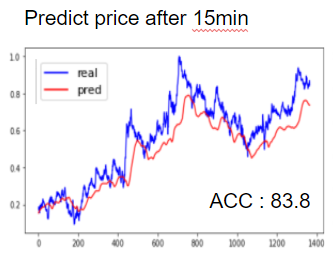
\includegraphics[width=0.8\linewidth]{latex/LSTM_15.PNG}
\end{center}
\label{fig:LSTM15}
\end{figure}

\begin{figure}[h!]
\begin{center}
\caption{Predicting the bitcoin price after 90 min using LSTM}
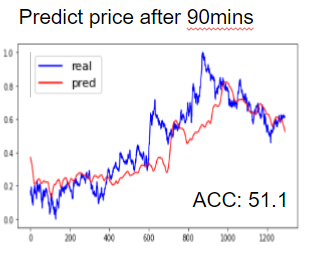
\includegraphics[width=0.8\linewidth]{latex/LSTM_90.PNG}
\end{center}
\label{fig:LSTM90}
\end{figure}

We have observed that although LSTM performs better for a shorter window, the Linear regression model has better accuracy of 64\%\ref{fig:linear90} when compared to LSTM's 51\%\ref{fig:LSTM90} when the window size goes to 90min. Out of all the regression models we have tried from scikit learn, the SGD regression model has the best accuracy for a 90 min window of around 80\%\ref{fig:sgd90}. This tells us that the normal regression model can solve some aspects of temporal latency compared to the neural network which uses has more variance and tries to over-fit the model.

\begin{figure}[h!]
\begin{center}
\caption{Predicting the bitcoin price after 90 min using Linear model}
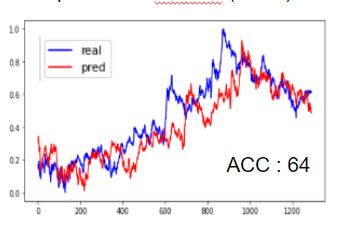
\includegraphics[width=0.8\linewidth]{latex/linear_90.PNG}
\end{center}
\label{fig:linear90}
\end{figure}

\begin{figure}[h!]
\begin{center}
\caption{Predicting the bitcoin price after 90 min using SGD regressor model}
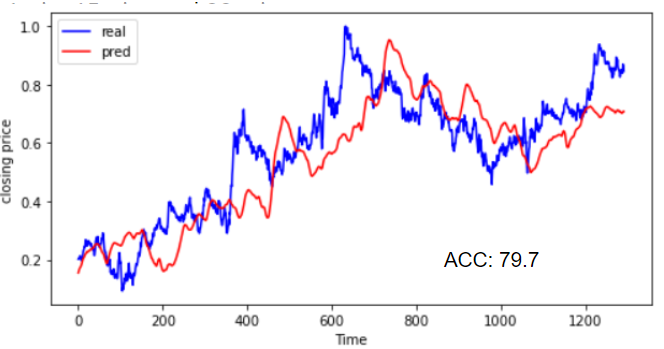
\includegraphics[width=0.8\linewidth]{latex/SGD_90.PNG}
\end{center}
\label{fig:sgd90}
\end{figure}


\subsection{Twitter data}
Twitter crypto hashtag keyword count is a metric we are using to do our correlation analysis based on the Tweet Volume Analysis.  We have created a set of exhaustive keywords to be identified among the tweet hashtags. We are using Twitter API, tweepy library, spark streaming to get the hashtag counts from Twitter and storing them in the google cloud storage for 10 min windows, We are also using Crypto compare API to get the real-time data of the cryptocurrency values. Currently, we are using the stored data from the 10min window of tweets and crypto compare API for correlation analysis and we haven't seen any strong correlation between the two. We think that lack of correlation is due to the time window being too short and using the count data just to observe the price change may not be relevant and we should be using it for a derived trend prediction. Overall that was our discovery through Tweet Volume Analysis. For Twitter Sentiment Analysis, we followed a similar set up procedure where we used the Twitter ApI, tweepy library, and spark streaming to stream the twitter data, but we also used the NLTK library to quantitatively score the Twitter Sentiment. We streamed a million tweets over a period of 90 days and compared it to the cryptocurrency price over the past 90 days using data from the CryptoCompare API. We assigned each tweet a sentiment score value as shown in Figure 12 and did a histogram distribution to observe the sentiment analysis correlation with the cryptocurrency price. The more positive score means greater positive sentiment while the more negative score means the greater negative sentiment. The correlation with the distribution and the cryptocurrency price trend seems to not exactly match the distribution was able to predict the rise, but the volatility was not able to be predicted. However, that was expected as discussed in the Related Work section. 

\begin{figure}[h!]
\begin{center}
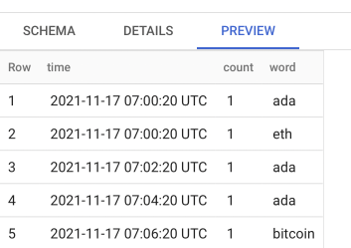
\includegraphics[width=0.8\linewidth]{latex/twitter.png}
\end{center}
   \caption{Twitter hashtag count data for crypto keywords}
\label{fig:long}
\label{fig:onecol}
\end{figure}

\begin{figure*}[h!]
\begin{center}
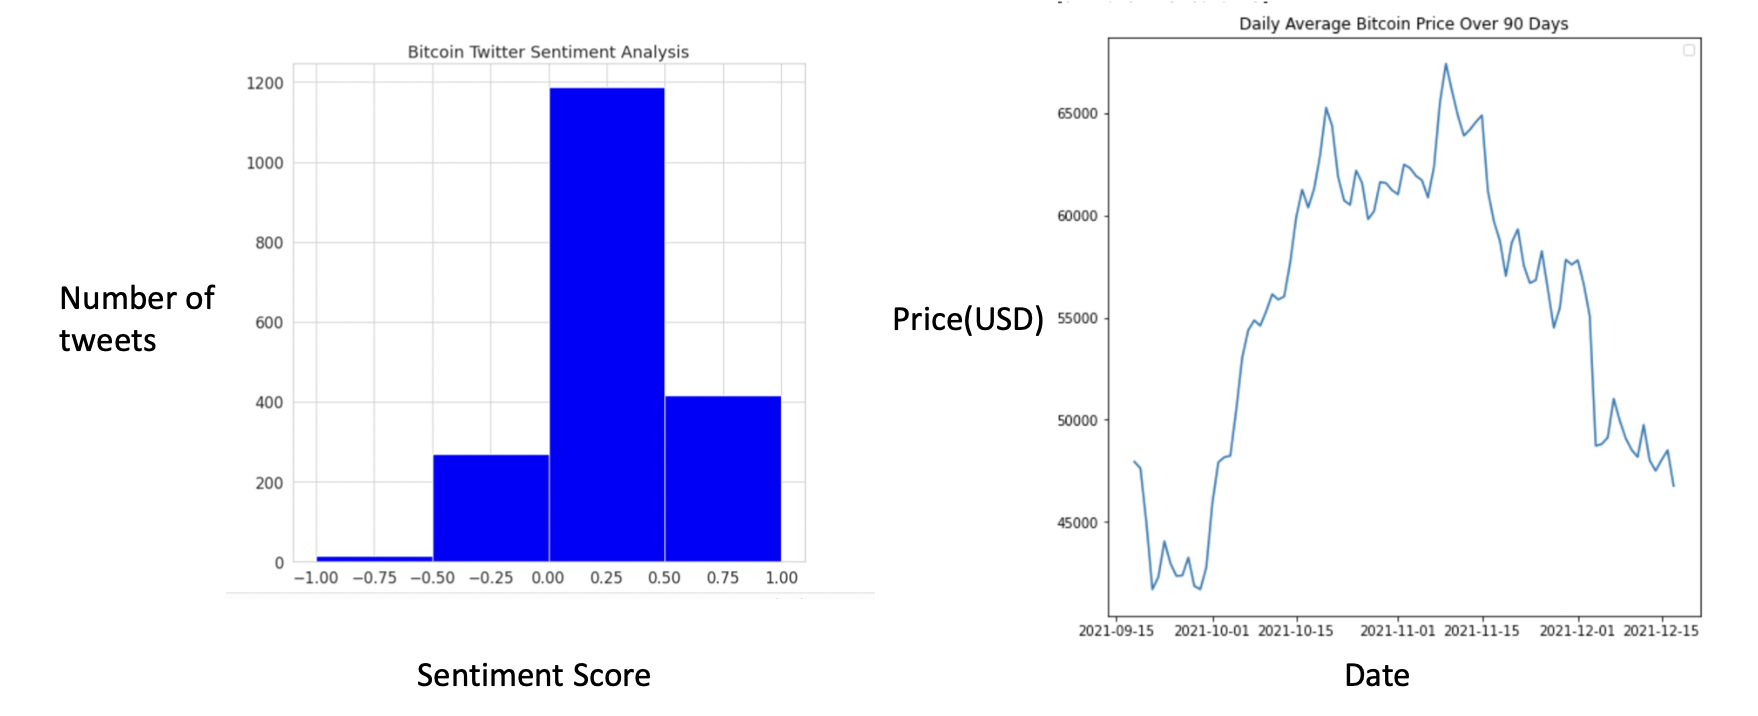
\includegraphics[width=0.8\linewidth]{latex/TSA.png}
\end{center}
   \caption{Twitter Sentiment Analysis Vs. Cryptocurrency Price}
\label{fig:long}
\end{figure*}


\begin{figure}[h!]
\begin{center}
\caption{Predicting the Ethereum price using H2O}
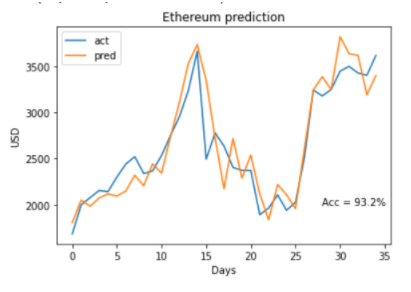
\includegraphics[width=0.8\linewidth]{latex/H2O_eth.PNG}
\end{center}
\label{fig:h2oeth}
\end{figure}

\begin{figure*}[h!]
\begin{center}
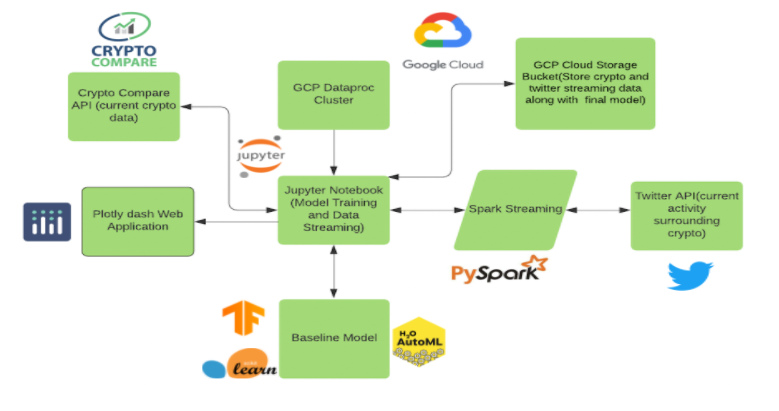
\includegraphics[width=0.8\linewidth]{latex/workflow_complete.PNG}
\end{center}
   \caption{The system workflow.}
\label{fig:short}
\end{figure*}



\subsection{Dynamic model}

All the experiments we have done for feature engineering and model selection has suggested the importance of a dynamic model. Hence, we have tested H2O's capability in maintaining the good accuracy consistently.

When H2O was used to train on the six month data of ethereum and tested against 30 days of future data. We have observed an accuracy of  93.2\%\ref{fig:h2oeth}. which is similar to bitcoin's 95.3\%\ref{fig:h2obtc}. The training time was set to only 10 minutes.


The best model, that generated the ethereum result is a gradient boost machine with 50 trees, average depth of 7 and average number of leaves as 80. which is different from the best model in case of bit coin which was multi layer perceptron. 

\begin{figure*}[h!]
\begin{center}
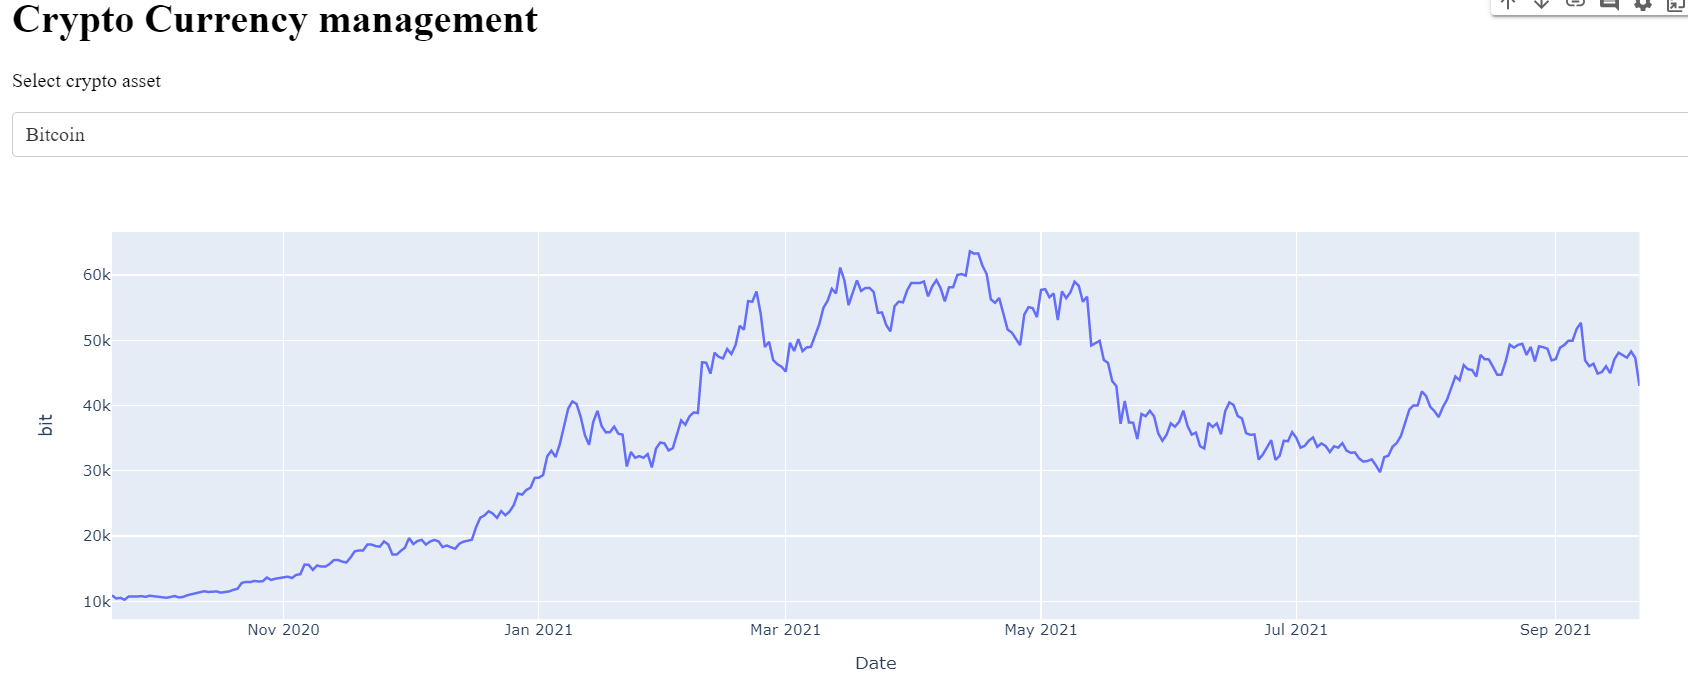
\includegraphics[width=0.8\linewidth]{latex/bitcoin_web app.PNG}
\end{center}
   \caption{Track multiple currencies from the drop down}
\label{fig:track}
\end{figure*}

\begin{figure*}[h!]
\begin{center}
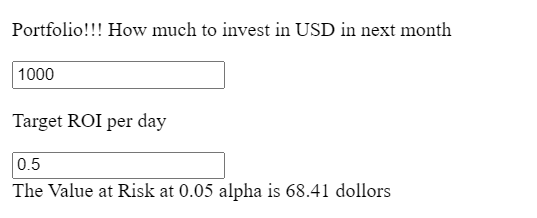
\includegraphics[width=0.8\linewidth]{latex/investment.PNG}
\end{center}
   \caption{User input the investment amount and desired return }
\label{fig:inv}
\end{figure*}

\begin{figure*}[h!]
\begin{center}
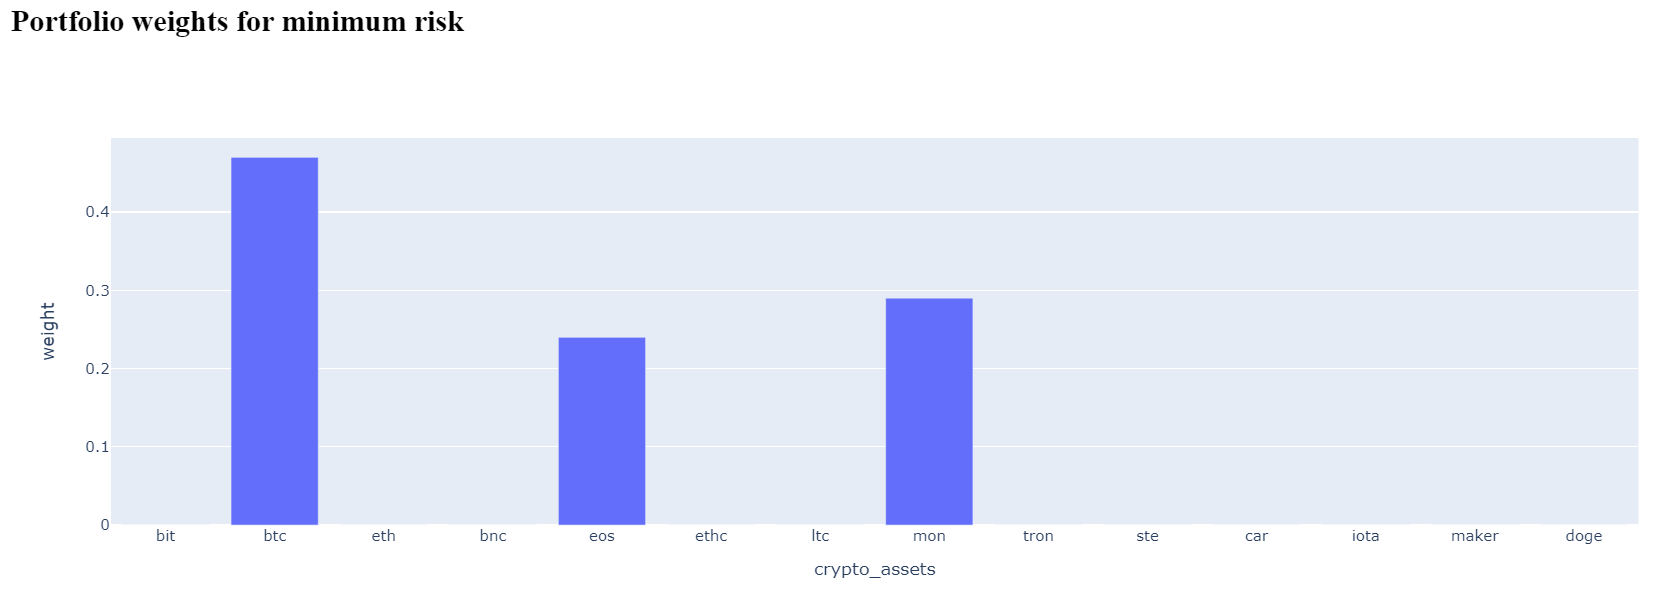
\includegraphics[width=0.8\linewidth]{latex/portfolio_min.PNG}
\end{center}
   \caption{weights for the least risk possible for the desired return}
\label{fig:weights}
\end{figure*}


Even if we compare the leader boards of bitcoin and ethereum, we can see that the top models are different for both the currencies\ref{tab:leader}. The stacked ensemble in the H2O is the combination of best performing models if 'best' is their in the name and also all the weak models are also tried during stacking and we could see 'All' in the name. Bitcoin's best models are mostly stacked ensemble models and MLP while best models of ethereum are all random forest models and some stacked ensemble models that are combination of random forests.This emphasises the need for dynamic model.

\begin{table}[h!]
\centering
 \begin{tabular}{ |p{2.5cm}|p{2.5cm}|}
 \hline
 \multicolumn{2}{|c|}{\textbf{Leader board}} \\
 \hline
 Bitcoin & Ethereum \\
 \hline
 MLP  & GBM \\
 \hline
 Stacked ensemble best-9 & Stacked ensemble best-3 \\
 \hline
  Stacked ensemble best-5 &  XRT-1 \\
 \hline
  Stacked ensemble all-3 &   Stacked ensemble best-3\\
 \hline
  Stacked ensemble best-4&   GBM\\
 \hline
  \end{tabular}
  \caption{leader board of bitcoin and ehtereum models}
 \label{tab:leader}
\end{table}


\subsection{portfolio analysis}
Different experiments were done by changing the desired return and investment values to calculate the weights of the portfolio. The results show that the algorithm has implicitly segregated the low risk and high risk crypto assets. When the desired ROI per day is given as  0.5\% \ref{fig:roi5}, it can be seen that the currencies like bitcoin cash, EOS and Monero have been given high weightages as they are very low risk and low return assets. when the desired ROI per day is increased to 1.5\%,\ref{fig:roi32} it can be seen that cardano has been given the highest weightage and both bitcoin and doge are added to the portfolio as they are high return assets with more risk. When the ROI is increased to 2\%\ref{fig:roi2}. it can be seen most of the investment going to doge as it is the asset with highest return and highest risk. The increase in the risk also can be seen from the increase in the value at risk value that was displayed from 68 to 94 dollars.

\section{System overview}

The system workflow is that it takes the real-time crypto data from "Crypto-compare API" and Tweepy library is used to access the Twitter API to fetch real-time tweets data upon which Tweet Volume Analysis and Twitter Sentiment Analysis are done. Although, the analysis is done currently the model isn't taking the new data as this feature is discarded. The last six months data is divided into training(5 months) and test(1 month) data set for the dynamic model training. The H2O AutoML tool is set to run for a maximum of 10 minutes. The model generates the model with the best cross-validation accuracy. Then the model is used to predict the next day's return. The portfolio algorithm is developed in R, that uses the package "quantprog" to solves the quadratic optimization for minimum variance. It uses "Performance Analytics" to calculate the value at risk which is the amount that could be at risk based on the investment value and desired return. It also uses "quantmod" for finanacial statistical vector calculations. All of the R code is wrapped using "rpy2" library that will convert this code into python callable function. This callable function is the input to the web app. The web application is created using plotly "dash" which can be used to develop interactive applications. It has HTML like components which could be used to set up layout for the web app. It is written on top of plotly.js and react.js. It has objects called Dash core components which could be used to create interactive components on web app. This web app is created in such a way that it takes the multiple currency close prices and displays as a interactive drop down that investor can use to track the multiple cryptocurrencies.\ref{fig:track}. The user is given a interactive text block where he inputs the amount he would like to invest, then he inputs the desired return per day.\ref{fig:inv} These two values will be used to calculate the weights of each of the crypto currencies in the portfolio that would achieve the desired return with the least risk possible.\ref{fig:weights} The portfolio algorithm also calculates value at risk part of his investment based on normal distribution and a confidence interval of 0.05. There are bottlenecks in the system when it comes to the API calls regarding streaming as there might be high latency depending on the frequency of the API calls.  However, they can be improved by running our model on a more powerful GPU once we are able to prove its validity in the long run to make justify the cost of an expensive GPU. The main improvement we can make regarding API streaming be it from CryptoCompare or Twitter is to make our code more robust and use methods such as caching to make our search calls execute faster. Currently, the web app doesn't have the out of range values handling and needs to be implemented.


\section{Conclusion}

The initial assessments that the other crypto datasets can be used to improve the prediction accuracy was not helpful as it is later observed that there is no improvement in the accuracy although we can see that there is a strong correlation between the cryptocurrencies in some time frames. To use this intelligence in future we have to use some freuqency based techniques like fpca to extract the value. The paper discusses why the dynamic model architecture is better compared to a single model that has high variance with respect to the training data and volatile data like crypto data should not be used with a single model architecture as changing the constraints like time period will make the model less effective. We also observed the literature favoured LSTM, which represents a deep learning model is effective in the short term windows but will not even be as effective as linear regression models when used  to predict well ahead in the future(change constraints) due to over-fitting. The observation to note here is the multi layer perceptron which is a deep learning model is the leader model when predicting bitcoin using H2O. This is due to its effectiveness on training for the given temporal data frame. hence, using this advantage dynamic model will consistently deliver even when the temporal data frame is moved. We have also learned that doing Tweet Volume Analysis and Twitter Sentiment Analysis provides a decent feature but increases the variance of the model, hence it is not included as a feature to the final model. Portfolio analysis has shown how risk could be minimised even in a high risk market such as crypto assets. It also provides users with the least risk portfolio for the same desired return. In turn it has segregated the cryptocurrencies with high risk from the low risk\ref{fig:roi2}\ref{fig:roi32}. In the future we would like to connect the APIs  with the model and implement this work flow on hadoop, so it can be scaled and serve large number of users. 




%-------------------------------------------------------------------------



{\small
\bibliographystyle{ieee_fullname}
\bibliography{egbib}
}

\section{contribution}

Siddartha Marella (sm4940) : 

1. Correlation analysis for usefulness of multiple currencies in crypto prediction.
2. LSTM and scikit model training for the crypto prediction.
3. H2O Automl dynamic model setup for crypto prediction
4. Portfolio algorithm for Risk minimization and portfolio creation.
5. Web app creation using dash for interactive usage.

Varun Jasti (vj2252) :  1. Models and Correlation Analysis Research for                                different implementations 
                        2. Set up Spark and live crypto Streaming
                        3. Google Cloud Setup 
                        4. Set up needed infrastructure to connect components of project through APIs 
                        5. Twitter Analysis Testing 
                        6. Prediction Calculations for different models        tested
                        
                        7. Literature Review 
\begin{table}[h!]
\centering
 \begin{tabular}{ |p{2.5cm}|p{1.5cm}|}
 \hline
 \multicolumn{2}{|c|}{\textbf{Quantiative contribution}} \\
 \hline
 Siddartha Marella(sm4940) & 67\%  \\
 \hline
 Varun Jasti(vj2252) & 33\%\\
 \hline
 \end{tabular}
  \caption{Contribution.}
 \label{tab:ADF-C}
\end{table}


\section{Appendix}

\begin{table}[h!]
\centering
 \begin{tabular}{ |p{2.5cm}|p{1.5cm}|p{1.5cm}|}
 \hline
 \multicolumn{3}{|c|}{\textbf{ADF - stationary test}} \\
 \hline
 Currency & Stationary & p-value \\
 \hline
 Bitcoin  & FALSE & 0.62 \\
 \hline
 Bitcoin cash  & FALSE & 0.12 \\
 \hline
 Binance coin  & FALSE & 0.89 \\
 \hline
 EOS  & FALSE & 0.49 \\
 \hline
 Ethereum classic  & FALSE & 0.48 \\
 \hline
 Ethereum  & FALSE & 0.14 \\
 \hline
 Litecoin  & FALSE & 0.22 \\
 \hline
 Monero  & FALSE & 0.66 \\
 \hline
 TRON  & FALSE & 1 \\
 \hline
 Stellar  & FALSE & 0.09 \\
 \hline
 Cardano  & FALSE & 0.69 \\
 \hline
  IOTA  & FALSE & 0.77 \\
 \hline
  Maker & FALSE & 0.14 \\
 \hline
  Dogecoin  & FALSE & 0.33 \\
 \hline
  \end{tabular}
  \caption{ADF- Stationary test for close prices in Q1-2021.}
 \label{tab:ADF-C}
\end{table}


\begin{table}[h!]
\centering
 \begin{tabular}{ |p{2.5cm}|p{1.5cm}|p{1.5cm}|}
 \hline
 \multicolumn{3}{|c|}{\textbf{ADF - stationary test}} \\
 \hline
 Currency & Stationary & p-value \\
 \hline
 Bitcoin  & TRUE & 0 \\
 \hline
 Bitcoin cash  & TRUE & 0 \\
 \hline
 Binance coin  & TRUE & 0\\
 \hline
 EOS  & TRUE & 0 \\
 \hline
 Ethereum classic  & TRUE & 0  \\
 \hline
 Ethereum  & TRUE & 0  \\
 \hline
 Litecoin  & TRUE & 0  \\
 \hline
 Monero  & TRUE & 0  \\
 \hline
 TRON  & TRUE & 0  \\
 \hline
 Stellar  & TRUE & 0  \\
 \hline
 Cardano  & TRUE & 0  \\
 \hline
  IOTA  & TRUE & 0  \\
 \hline
  Maker & TRUE & 0  \\
 \hline
  Dogecoin  & TRUE & 0  \\
 \hline
  \end{tabular}
  \caption{ADF- Stationary test for close prices in Q1-2021 after log-return calculation.}
 \label{tab:ADF1-C}
\end{table}

\begin{figure}[h!]
\begin{center}
\caption{Predicting the bitcoin price after 1 min using LSTM}
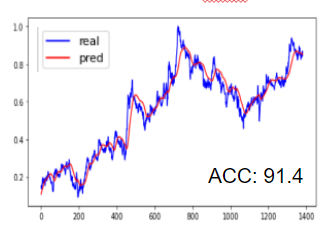
\includegraphics[width=0.8\linewidth]{latex/LSTM_1min.PNG}
\end{center}
\label{fig:LSTM1}
\end{figure}

\begin{figure*}[h!]
\begin{center}
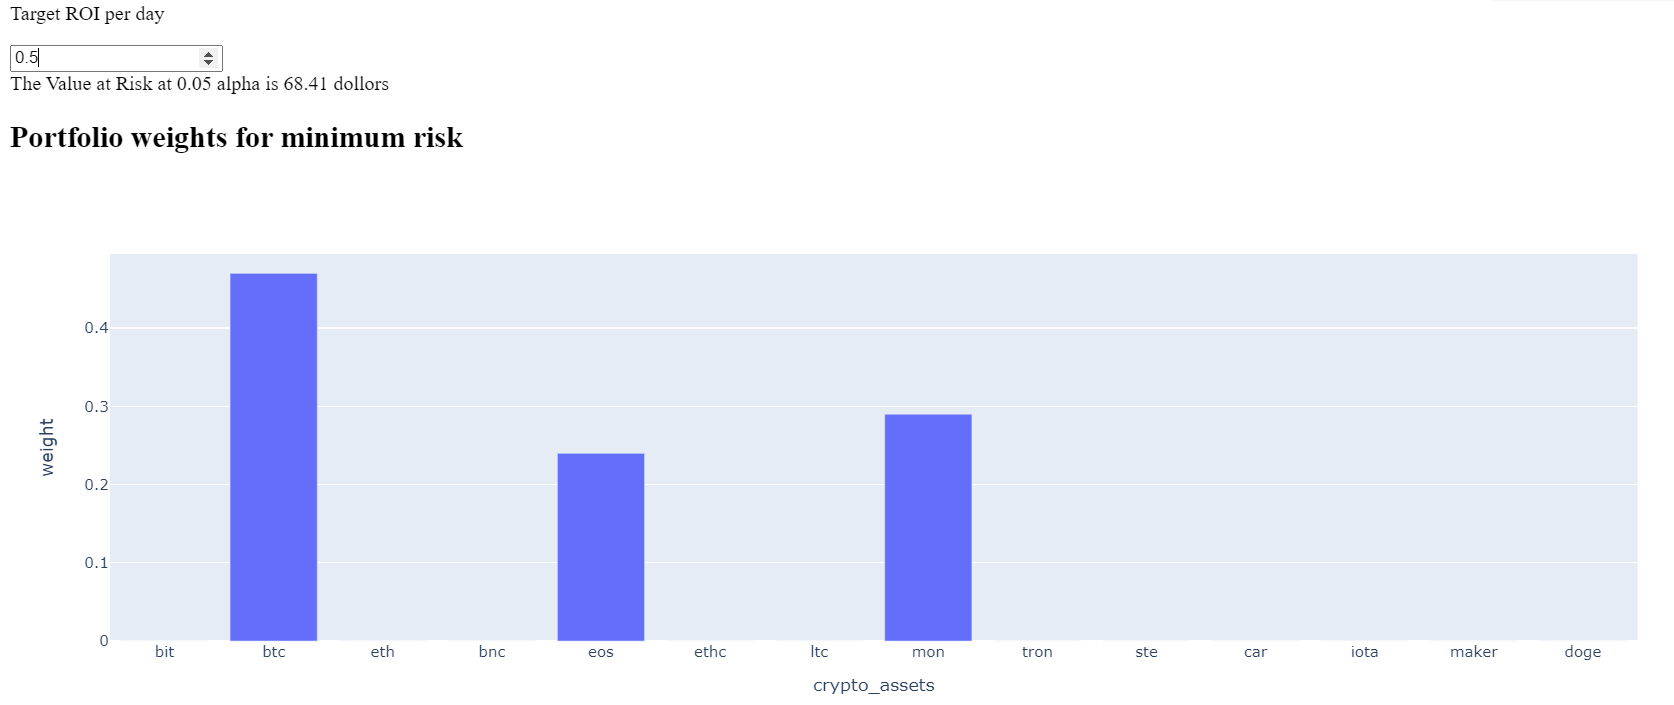
\includegraphics[width=0.8\linewidth]{latex/roi5.PNG}
\end{center}
   \caption{weights for the least risk possible for the return of 0.5 per day}
\label{fig:roi5}
\end{figure*}

\begin{figure*}[h!]
\begin{center}
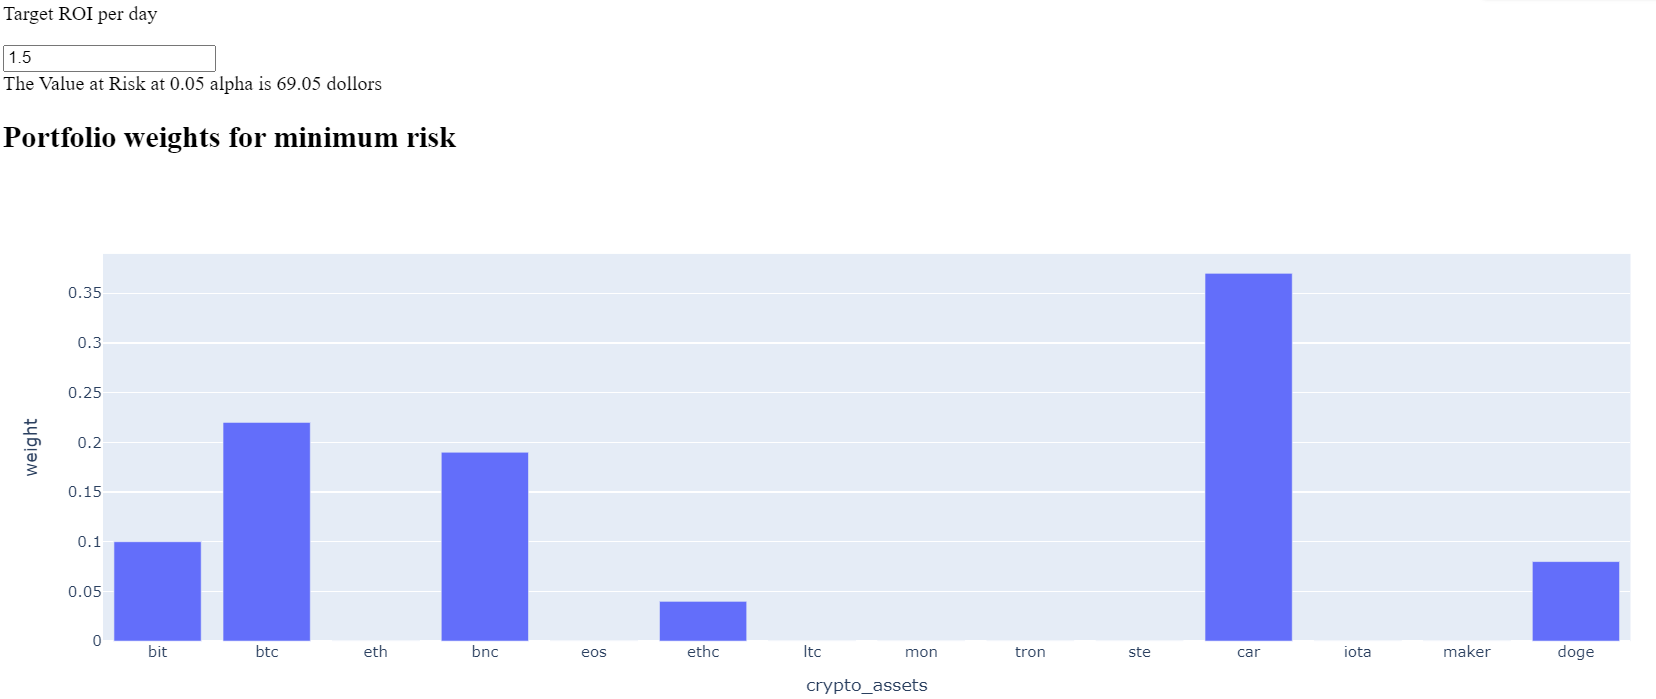
\includegraphics[width=0.8\linewidth]{latex/roi32.PNG}
\end{center}
   \caption{weights for the least risk possible for the return of 1.5 per day}
\label{fig:roi32}
\end{figure*}

\begin{figure*}[h!]
\begin{center}
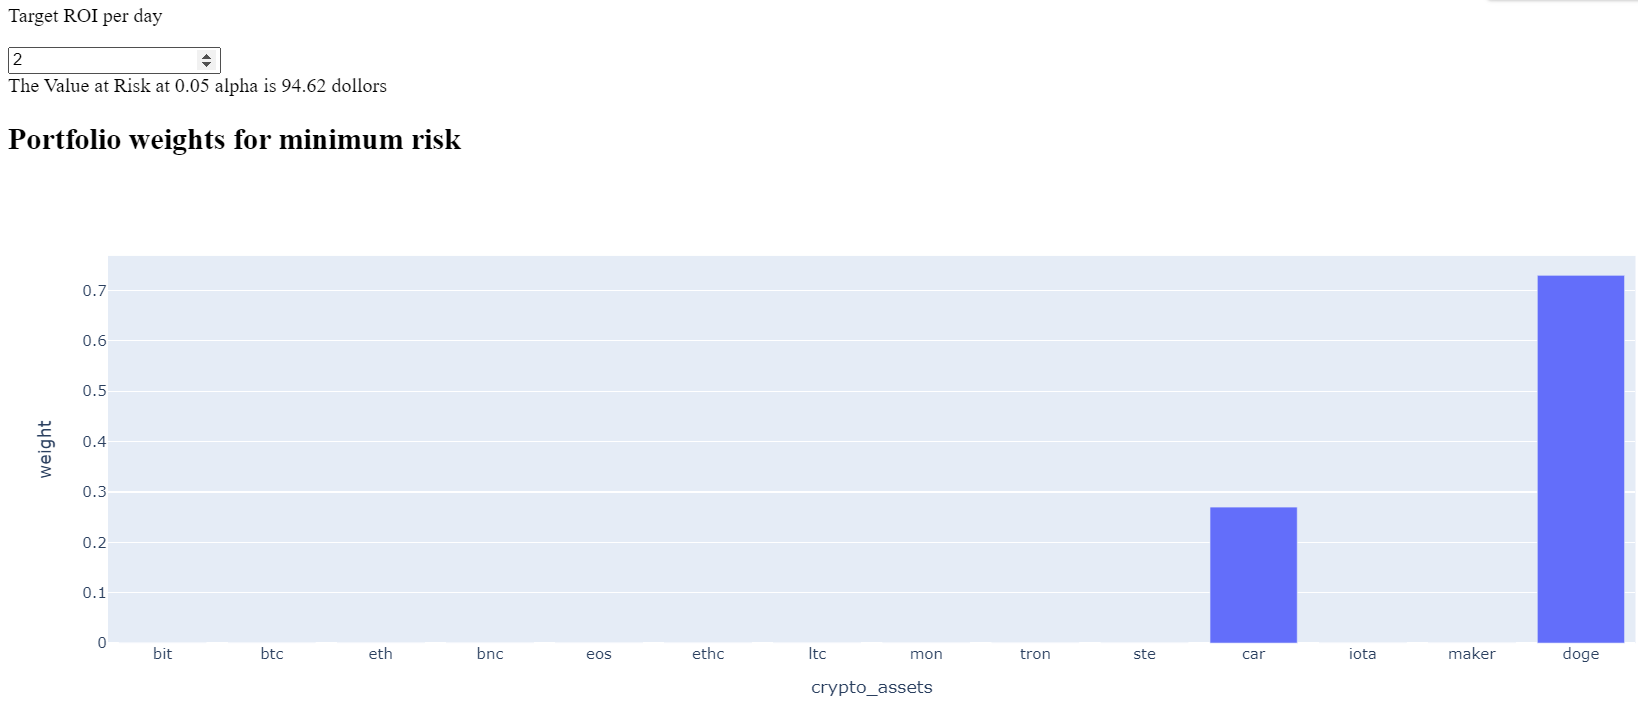
\includegraphics[width=0.8\linewidth]{latex/roi2.PNG}
\end{center}
   \caption{weights for the least risk possible for the return of 2 per day}
\label{fig:roi2}
\end{figure*}

\end{document}
